%% The Rice SIAM chapter 50-digit challenge (2005), corrected edition.
%% Build:  make pdf      (needs figs/, tables/ and snippets/, all written by
%%                        make check, which runs code/paper.py)
\documentclass[final]{siamltex}
\usepackage{amsmath}
\usepackage{amssymb}
\usepackage[pdftex]{graphicx}

\parskip = 5pt minus 1pt
\raggedbottom

\input{tables/numbers}

\newcommand{\bp}{\mathbf{p}}
\newcommand{\bv}{\mathbf{v}}
\newcommand{\bw}{\mathbf{w}}
\newcommand{\bn}{\mathbf{n}}
\newcommand{\diam}{\hfill$\diamond$}

\title{The Rice SIAM chapter 50-digit challenge\thanks{Written in 2005;
this is a corrected edition. Section 6 of the original gave the wrong
answer, and Sections 3 and 5 drew the wrong conclusion from a right one.
Section 1.1 lists everything that changed. The code is at
\texttt{code/}, and \texttt{make check} reproduces every number below.}}
\author{Thomas Schmelzer\thanks{Computing Laboratory, Oxford University.
The author was supported by the Rhodes Trust.}}

\begin{document}
\maketitle

\begin{abstract}
The Rice University SIAM student chapter published five new 10-digit
problems. The intention is that Rice students solve every problem to as many
digits of precision as possible. Archetype for this idea was a similar
competition which culminated in a beautiful book \cite{bornemann}. This note
gives my solutions, an alternative sixth problem, and an appendix on the
integral of $\sin^2(\tan(\tan(\pi x)))$, which is where the mathematics is.
\end{abstract}

\section{Introduction}
Each of the questions below has an answer that is a single real number. The
problems should be answered in the form $d_1.d_2\ldots d_{10}\times 10^p$,
$d_1 \neq 0$, where the exponent must be correct but does not count toward
the number of correct digits and $d_{10}$ is obtained by rounding.

\begin{enumerate}
\item Two players each control one knight at opposite corners on an
$8\times 8$ chessboard. They simultaneously try to move their respective
pieces to an open square, using the L-shaped jump of the knight. Each of the
valid jumps for either of the knights has equal probability of occurring.
However if the two players choose to move their knights to the same square,
they instead leave their pieces where they are and the turn is passed. What
is the probability of at least one knight being at one of the four corners
of the chessboard after 2005 turns?

\item A photon lies in the $x$-$y$ plane trapped between two elliptical
mirrors given by the equations $4x^2+y^2=4$ and $9x^2+16y^2=144$. At time
$t=0$ the photon begins heading due north from position $(2,0)$ with unit
speed. How far is the photon from the origin at time $t=60$?

\item Define the polynomial $p(x) = \sum_{k=0}^{10,000} a_k x^k$, where
$a_k$ is the $(k+1)$st prime number. What is the magnitude of the root of
$p$ nearest the origin?

\item A point mass is at rest at the origin in the $x$-$y$ plane. At time
$t=0$ the four other point masses listed in the table below are traveling
clockwise with unit speed perpendicular to the radial direction. Each mass
$m_i$ attracts each other mass $m_j$ with a gravitational force of magnitude
$F_{ij} = m_i m_j / r^2$, where $r$ is the distance of $m_i$ from $m_j$. If
these are the only forces present, how far from the origin is point $p_4$ at
time $t=5$?

\begin{center}
\begin{tabular}{c@{\hspace{1.5em}}r@{\hspace{1.5em}}r@{\hspace{1.5em}}r@{\hspace{1.5em}}r@{\hspace{1.5em}}r}
\hline
Point & $p_0$ & $p_1$ & $p_2$ & $p_3$ & $p_4$\\
\hline
$m_i$ & 10 & 1 & 1 & 1 & 1\\
$x_i$ & 0 & 0 & 2 & 0 & $-4$\\
$y_i$ & 0 & 1 & 0 & $-3$ & 0\\
\hline
\end{tabular}
\end{center}

\item A sphere with unit radius centered at the origin in an $(x,y,z)$
coordinate system is missing the part of its surface with $z$-coordinate
greater than $3/4$. Two uniform balls with radius $1/4$ and unit mass are at
rest at positions $(1/2,1/8,0)$ and $(0,1/2,0)$ inside the open
``fishbowl.'' At time $t=0$, the balls are imparted with unit velocities
toward the origin. What is the distance between the centers of the two balls
at $t=10$ if all collisions are completely elastic and there are no external
forces?
\end{enumerate}

Each of the next sections covers one problem, and the answers are collected
in Section 7. I could not resist adding a suggestion for a sixth problem,
and in an appendix I discuss the integral
\[
   \int_0^1 \sin^2\bigl(\tan(\tan(\pi x))\bigr)\,dx ,
\]
which is a problem I had some fun with.

\subsection{What changed in this edition}
The original note is twenty years old and three of its sections needed work.

\emph{Section 6 was wrong.} The two balls were made to exchange their whole
velocity vectors on impact, which is the head-on case. The answer to
Problem 5 is \bowlanswer, not the \bowlold\ submitted in 2005.

\emph{Section 3 drew the wrong moral.} A table of Mathematica runs was read
as showing that ``a loss of 43 digits is unavoidable'' in an elliptic
billiard. What that table measured was the worst-case bound significance
arithmetic carries along, not the conditioning of the problem, which costs
about one and a half digits over the whole flight.

\emph{Section 5 certified its answer the wrong way.} It perturbed the
initial data and watched the spread. That measures conditioning; the error
of the integration is shared by all those runs and cannot show up in their
spread. Both experiments are now run, and separately.

\emph{Section 4 had a gap.} The bound that licensed truncating the
polynomial controls function values and says nothing about where the roots
are. Rouch\'e's theorem fills it in two lines.

The MATLAB and Mathematica of 2005 has been rewritten in Python, and the
listings in this note are extracted from the files that produce its numbers,
so the two cannot drift apart. Every figure, table and displayed constant
comes out of \texttt{make check}. I have also fixed the typography and the
typing, of which there was a good deal.

\section{A Markov chain}
We analyse the random walk of two knights on a chessboard.

\noindent\textbf{Problem.} \emph{Two players each control one knight at
opposite corners on an $8\times 8$ chessboard\ldots\ What is the probability
of at least one knight being at one of the four corners of the chessboard
after 2005 turns?} \diam

\begin{figure}[htb]
\centerline{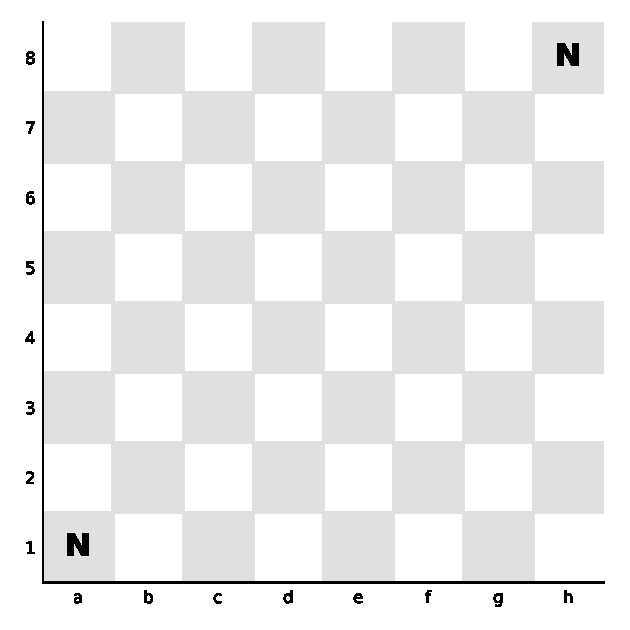
\includegraphics[width=0.42\textwidth]{figs/board}}
\caption{The knights start in opposite corners, on squares of the same
colour.}
\end{figure}

To each square we assign a number $p = 8(i-1) + j$, where $i$ is the row and
$j$ the column, so the knights start on squares 1 and 64. A pair of occupied
squares is a state, numbered $s = 64(p^{(1)}-1) + p^{(2)}$, and there are
$64^2 = 4096$ of them. Many are unreachable. Both knights move or, when they
choose the same square, neither does, so the two squares keep the colour
they started with and only the same-coloured pairs occur.

From a square $p$ the knight can reach:

\begin{verbatim}
def moves(p):
    """The squares a knight standing on square p can jump to."""
    row, col = divmod(p - 1, 8)
    jumps = ((2, -1), (2, 1), (1, -2), (1, 2),
             (-2, -1), (-2, 1), (-1, -2), (-1, 2))
    return [8 * (row + dr) + (col + dc) + 1
            for dr, dc in jumps
            if 0 <= row + dr < 8 and 0 <= col + dc < 8]
\end{verbatim}


Let the first knight have $n_1$ squares available and the second $n_2$,
where in each case the square held by the other knight is excluded. The
players choose independently, so each of the $n = n_1 n_2$ pairs has
probability $1/n$. If $m$ of those pairs name the same square, the turn is
passed, and the chain stays where it is with probability $m/n$. This defines
a matrix $A$:

\begin{verbatim}
def transition():
    """The column-stochastic matrix of the chain on the 4096 states.

    Each player picks uniformly among the squares his knight can
    reach, the square held by the other knight excluded.  If both
    pick the same square nobody moves and the turn is passed, which
    is the diagonal entry.
    """
    A = sp.lil_matrix((64 * 64, 64 * 64))
    for i in range(1, 65):
        for j in range(1, 65):
            if i == j or colour(i) != colour(j):
                continue     # unreachable: they move together
            to_i = [q for q in moves(i) if q != j]
            to_j = [q for q in moves(j) if q != i]
            n = len(to_i) * len(to_j)
            passed = 0
            for a in to_i:
                for b in to_j:
                    if a == b:
                        passed += 1
                    else:
                        A[state(a, b) - 1, state(i, j) - 1] += 1 / n
            A[state(i, j) - 1, state(i, j) - 1] += passed / n
    return A.tocsc()
\end{verbatim}


$A$ is $4096\times 4096$ with \knightsnnz\ nonzero entries, all nonnegative,
and the entries of a reachable column sum to one. Starting from the state
$s = 64$ we want $v = A^{2005}e_{64}$, whose $i$th entry is the probability
of being in state $i$ after 2005 turns. We do not form $A^{2005}$:

\begin{verbatim}
def corner_indicator():
    """1 on every state with at least one knight on a corner."""
    w = np.zeros(64 * 64)
    for a in range(1, 65):
        for b in range(1, 65):
            if a in CORNERS or b in CORNERS:
                w[state(a, b) - 1] = 1.0
    return w


def solve():
    A = transition()
    v = np.zeros(64 * 64)
    v[state(*START) - 1] = 1.0
    for _ in range(TURNS):
        v = A @ v                      # not A**2005 applied to v
    w = corner_indicator()
    return A, v, w @ v
\end{verbatim}


Summing the entries of $v$ gives $1$ to fourteen places, which is the
arithmetic checking itself. Adding the entries of $v$ over the states with a
knight on a corner gives
\[
   \knightslong .
\]

\begin{figure}[htb]
\centerline{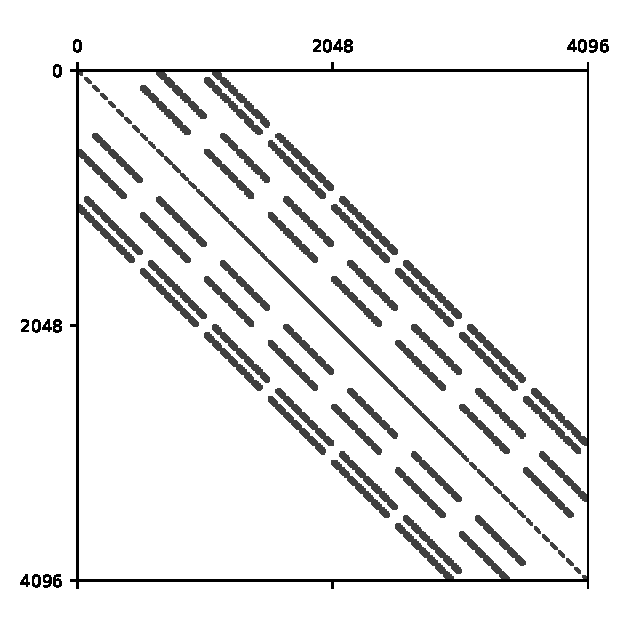
\includegraphics[width=0.46\textwidth]{figs/spy}}
\caption{The \knightsnnz\ nonzero entries of $A$.}
\end{figure}

The matrix has an eigenvalue exactly $1$, and the rest lie in a disc of
radius $\knightssecond$ about the origin. Deleting the unreachable rows and
columns leaves a column-stochastic matrix, whose dominant eigenvector $u_1$
is the stationary distribution; since $e_{64}^{H}u_1 \neq 0$ and
$\|v\|_1 = 1$,
\[
   p \;=\; \frac{w^{H}u_1}{\|u_1\|_1} ,
\]
with $w$ the indicator of the corner states. This costs one eigenvector
instead of 2005 matrix-vector products and agrees with the walk to twelve
digits.

It also says something the walk does not. The subdominant eigenvalue has
modulus \knightssecond, and $\knightssecond^{2005} \approx \knightsdecay$,
so after 2005 turns nothing whatever is left of the initial condition: the
answer is the stationary probability, and it would be the same after 300
turns or 300\,000. The 2005 in the question is decoration. What does matter
is the colour of the starting squares, since the chain never leaves the
component it starts in.

Hence I submit as solution for this problem
\[
   \knightsanswer .
\]

\section{A photon trap}
We chase a photon trapped between two elliptic mirrors.

\noindent\textbf{Problem.} \emph{A photon lies in the $x$-$y$ plane trapped
between two elliptical mirrors\ldots\ How far is the photon from the origin
at time $t=60$?} \diam

The inner mirror $4x^2+y^2=4$ has semi-axes $a=1$, $b=2$ and the outer
mirror $9x^2+16y^2=144$ has $a=4$, $b=3$. A moving photon was also an issue
in the original competition, where Wagon discusses it in a chapter of
\cite{bornemann}.

Between reflections the photon travels in a straight line, so the time to
the next mirror is the smallest positive root of a quadratic:

\begin{verbatim}
def hit(p, v, a, b, leaving):
    """Smallest t > 0 with (px+t vx)^2/a^2 + (py+t vy)^2/b^2 = 1.

    `leaving` says the photon is sitting on this mirror, so t = 0 is a
    root: divide it out rather than filter roots by a threshold.
    """
    qa = v[0] ** 2 / a ** 2 + v[1] ** 2 / b ** 2
    qb = 2 * (p[0] * v[0] / a ** 2 + p[1] * v[1] / b ** 2)
    if leaving:
        t = -qb / qa
        return t if t > 0 else mp.inf
    qc = p[0] ** 2 / a ** 2 + p[1] ** 2 / b ** 2 - 1
    disc = qb * qb - 4 * qa * qc
    if disc < 0:
        return mp.inf
    root = mp.sqrt(disc)
    ts = [t for t in ((-qb - root) / (2 * qa),
                      (-qb + root) / (2 * qa)) if t > 0]
    return min(ts) if ts else mp.inf
\end{verbatim}


The one delicate point is the root at $t=0$. After a reflection the photon
sits on the mirror it just left, so that quadratic has a root there, and a
routine returning the smallest positive root can return a
rounding-error-sized one instead of the flight. Rather than reject roots
below a threshold --- which is a tolerance, and tolerances have to be tuned
--- we divide the known root out. The remaining root is $-b/a$ exactly.

At a reflection the tangential part of the velocity survives and the normal
part changes sign. The outward normal of $x^2/a^2+y^2/b^2=1$ at $\bp$ is
$(p_x/a^2,\,p_y/b^2)$, which is all we need:

\begin{verbatim}
def reflect(p, v, a, b):
    """Specular reflection at p on the ellipse with semi-axes a, b.

    The outward normal of x^2/a^2 + y^2/b^2 = 1 at p is
    (px/a^2, py/b^2); the tangential part of v survives and the
    normal part changes sign.
    """
    n = (p[0] / a ** 2, p[1] / b ** 2)
    scale = mp.sqrt(n[0] ** 2 + n[1] ** 2)
    n = (n[0] / scale, n[1] / scale)
    s = 2 * (v[0] * n[0] + v[1] * n[1])
    return (v[0] - s * n[0], v[1] - s * n[1])
\end{verbatim}


The flight is then a loop over events:

\begin{verbatim}
def fly(dps, shift=0, trace=False):
    """Distance from the origin at t = 60, at dps working digits."""
    mp.mp.dps = dps
    p = (mp.mpf(START[0]) + shift, mp.mpf(START[1]))
    v = (mp.mpf(DIRECTION[0]), mp.mpf(DIRECTION[1]))
    path, on, bounces, rem = [p], None, 0, mp.mpf(TEND)
    while rem > 0:
        dt, k = min((hit(p, v, a, b, on == i), i)
                    for i, (a, b) in enumerate(MIRRORS))
        dt = min(dt, rem)
        p, rem = (p[0] + dt * v[0], p[1] + dt * v[1]), rem - dt
        if trace:
            path.append(p)
        if rem > 0:
            v = reflect(p, v, *MIRRORS[k])
            on, bounces = k, bounces + 1
    return dict(distance=mp.sqrt(p[0] ** 2 + p[1] ** 2),
                bounces=bounces, path=path)
\end{verbatim}


\begin{figure}[htb]
\centerline{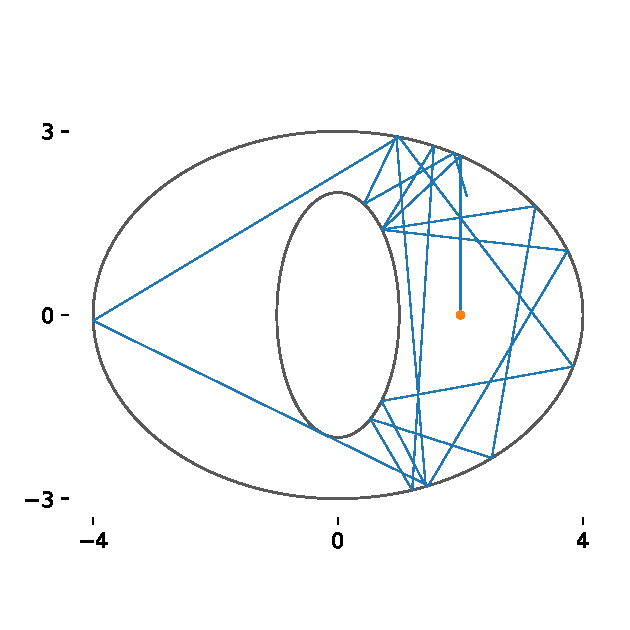
\includegraphics[width=0.58\textwidth]{figs/mirrors}}
\caption{The path of the photon over $0 \le t \le 60$: \photonbounces\
reflections, from the marked starting point.}
\end{figure}

\subsection{How ill-conditioned is it, really}
Reflection off a curved mirror is the textbook amplifier of small
differences, and the 2005 edition of this note ran the computation in
Mathematica at a range of precisions, watched the number of certified digits
fall far below the number carried, and concluded that ``a loss of 43 digits
is unavoidable.''\footnote{That conclusion was wrong, and the paragraph
around it has been replaced. The submitted answer was not affected.}

That is not what the experiment showed. Mathematica's significance
arithmetic carries an error bound along with each number and reports only
the digits that bound can certify; the bound is worst-case and accumulates
through every \texttt{Solve} and every \texttt{Inverse}. What the table
measured was the growth of that bound, not the sensitivity of the answer.

Carrying a fixed number of digits instead, and comparing against a run at
140 digits, gives Table 3.1: the loss is a digit and a half, and it does not
grow with the precision carried.

\begin{table}[htb]
\centerline{\input{tables/photon}}
\caption{Correct digits in $|\bp(60)|$ against working precision.}
\end{table}

The direct measurement agrees. Displacing the starting point by $\delta$
moves the answer by about $\photonamp\,\delta$, uniformly for $\delta$ from
$10^{-40}$ down to $10^{-15}$: over \photonbounces\ reflections the
amplification is a factor of \photonamp, not $10^{43}$. The billiard is
mildly ill-conditioned, as promised, and that is all. Twelve working digits
suffice for the ten the competition asks for; \photonlong\ is what 140
digits give, of which
\[
   \photonanswer
\]
is what I submit.

\section{An eigenvalue problem}
We compute the root nearest the origin of a polynomial of degree 10\,000.

\noindent\textbf{Problem.} \emph{Define the polynomial
$p(x) = \sum_{k=0}^{10,000} a_k x^k$, where $a_k$ is the $(k+1)$st prime
number. What is the magnitude of the root of $p$ nearest the origin?} \diam

The roots of a polynomial are the eigenvalues of its companion matrix, and a
degree-10\,000 companion matrix is more than this problem deserves. The
coefficients grow slowly --- $a_{10000} = \polyleading$ --- so for small $|x|$
the tail contributes very little, and we work with the truncation
$p_M(x) = \sum_{k=0}^{M}a_k x^k$ at $M=\polytruncated$:

\begin{verbatim}
def companion(coefficients):
    """Companion matrix of the monic multiple of the polynomial.

    coefficients[k] multiplies x^k, so the leading one is last.
    """
    a = np.array(coefficients, dtype=float)
    a = -a[:-1] / a[-1]
    n = len(a)
    A = np.zeros((n, n))
    A[0] = a[::-1]
    A[1:, :-1] = np.eye(n - 1)
    return A
\end{verbatim}


On the circle $|x| = 0.82$ every omitted term is at most
$a_{10000}\,0.82^{M+1}$, and there are fewer than 10\,000 of them:

\begin{verbatim}
def tail_bound(M=TRUNCATION, radius=CIRCLE):
    """A bound for |p - p_M| on |x| = radius.

    The coefficients increase, so every one of the omitted terms is at
    most a_10000 radius^(M+1).
    """
    mp.mp.dps = 40
    terms = DEGREE - M
    return terms * PRIMES[DEGREE] * radius ** (M + 1)
\end{verbatim}


which gives $|p - p_M| \le \polytail$ there.

\subsection{Why the truncation is legitimate}
The bound above controls the \emph{values} of $p - p_M$. The question asks
for a \emph{root}, and a small perturbation of a function is not by itself a
small perturbation of its zeros; the 2005 note passed over this.\footnote{A
gap in the original argument, filled here. The answer is unchanged.} What
closes the gap is Rouch\'e's theorem, which needs one more number: the
minimum of $|p_M|$ on the same circle.

\begin{verbatim}
def minimum_modulus(M=TRUNCATION, radius=CIRCLE, samples=4096):
    """min |p_M| on the circle of the given radius.

    Sampled, then polished by a local search: the modulus of a
    polynomial has no flat minima on a circle, so a fine sample finds
    every basin.
    """
    mp.mp.dps = 40
    coefficients = [mp.mpf(q) for q in PRIMES[:M + 1]][::-1]
    def modulus(theta):
        z = radius * mp.expjpi(2 * theta)
        return abs(mp.polyval(coefficients, z))
    grid = [(modulus(mp.mpf(j) / samples), mp.mpf(j) / samples)
            for j in range(samples)]
    value, theta = min(grid)
    step = mp.mpf(1) / samples
    for _ in range(60):
        step /= 2
        for candidate in (theta - step, theta + step):
            trial = modulus(candidate)
            if trial < value:
                value, theta = trial, candidate
    return value
\end{verbatim}


That minimum is \polyfloor, larger than \polytail\ by sixteen orders of
magnitude, so $|p-p_M| < |p_M|$ on $|x| = 0.82$ and $p$ and $p_M$ have the
same number of zeros inside. The truncation has \polyinside, a conjugate
pair, and therefore so does $p$; the root nearest the origin is one of them,
and no root of $p$ hides in the disc unaccounted for.

\begin{figure}[htb]
\centerline{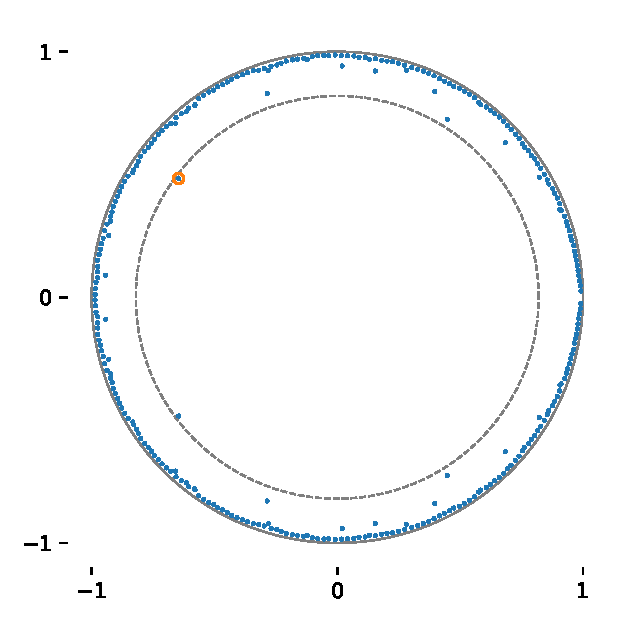
\includegraphics[width=0.52\textwidth]{figs/spectrum}}
\caption{The spectrum of the companion matrix of $p_{\polytruncated}$, with
the circles of radius $1$ and $0.82$. The nearest root is circled.}
\end{figure}

An eigenvalue of the truncated companion matrix is now a starting point
rather than an answer, and two Newton steps on the full polynomial settle
it:

\begin{verbatim}
def polish(seed, dps=50):
    """Newton on the full degree-10000 polynomial, from a seed."""
    mp.mp.dps = dps
    a = [mp.mpf(q) for q in PRIMES][::-1]
    d = [a[i] * (DEGREE - i) for i in range(DEGREE)]
    return mp.findroot(lambda x: mp.polyval(a, x) / mp.polyval(d, x),
                       mp.mpc(seed), tol=mp.mpf(10) ** -40)
\end{verbatim}


The root is a conjugate pair,
\[
   \polyreal + \polyimag\,i ,
\]
of magnitude \polylong, so I submit
\[
   \polyanswer .
\]

\section{A five-body problem}
The paths of five planets in a flat universe are determined by numerical
integration.

\noindent\textbf{Problem.} \emph{A point mass is at rest at the origin\ldots\
how far from the origin is point $p_4$ at time $t=5$?} \diam

Identify the phase space with $\mathbb{C}^{10}$: let $u \in \mathbb{C}^5$
hold the positions and $v \in \mathbb{C}^5$ the velocities, so that
\begin{equation}\label{eq:planets}
   \frac{d}{dt}\begin{pmatrix} u \\ v\end{pmatrix}
   = \begin{pmatrix} v \\ a\end{pmatrix} ,
   \qquad
   a_i = \sum_{j \neq i} m_j \frac{u_j - u_i}{|u_j - u_i|^3} ,
\end{equation}
the second equation being Newton's law with the masses divided out.

\begin{verbatim}
def field(u, v, masses=MASSES):
    """The acceleration of each mass, positions as complex numbers."""
    a = np.zeros(len(u), dtype=complex)
    for i in range(len(u)):
        for j in range(len(u)):
            if i != j:
                d = u[j] - u[i]
                a[i] += masses[j] * d / abs(d) ** 3
    return a
\end{verbatim}


The initial velocities are clockwise, of unit length and perpendicular to
the radius, so $u = (0, i, 2, -3i, -4)$ and $v = (0, 1, -i, -1, i)$.
Equation \eqref{eq:planets} is not stiff and the flight is short; a good
explicit method does it in a few seconds.

\begin{verbatim}
def integrate(rtol, shift=0.0, method="DOP853"):
    """|u_4(5)|, from a start optionally displaced by shift."""
    u0 = np.array(POSITIONS, dtype=complex)
    u0[WATCHED] += shift
    y0 = np.concatenate([u0.real, u0.imag,
                         np.real(VELOCITIES), np.imag(VELOCITIES)])

    def rhs(t, y):
        u = y[:5] + 1j * y[5:10]
        v = y[10:15] + 1j * y[15:]
        a = field(u, v)
        return np.concatenate([v.real, v.imag, a.real, a.imag])

    s = solve_ivp(rhs, [0, TEND], y0, method=method,
                  rtol=rtol, atol=1e-17)
    y = s.y[:, -1]
    return abs(complex(y[WATCHED], y[5 + WATCHED])), s.nfev
\end{verbatim}


\begin{figure}[htb]
\centerline{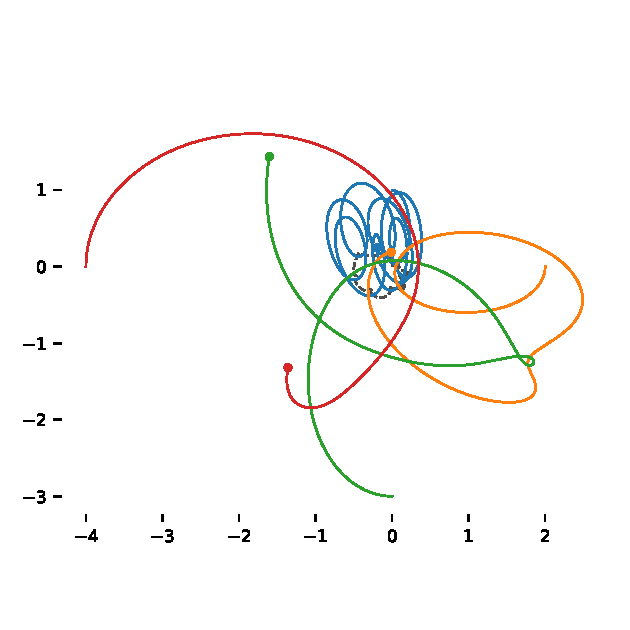
\includegraphics[width=0.56\textwidth]{figs/orbits}}
\caption{The five paths over $0 \le t \le 5$. The heavy mass, dashed, barely
moves; the closest any pair comes is \planetsseparation.}
\end{figure}

\subsection{How do we know ten digits are right}
The 2005 note asked this question and answered it by perturbing the initial
position of the fifth mass by about $10^{-16}$, repeating the integration
ten times, and reporting that the first ten digits agreed every
time.\footnote{The experiment was the wrong one; this subsection replaces
it. The submitted answer was right, by a margin of one unit in the tenth
digit.}

That experiment cannot answer the question. Every one of those runs used the
same solver at the same tolerance, so they share their discretisation error
almost exactly; what varies between them is the response to the data, and
what is being asked about is the error of the method. A spread of $10^{-10}$
across the ten runs tells us the problem amplifies the data by about
$\planetsamp$ over five time units --- worth knowing, and not an answer to
the question asked.

The experiment that does answer it varies the tolerance:

\begin{table}[htb]
\centerline{\input{tables/planets}}
\caption{$|u_4(5)|$ against the tolerance asked of the integrator.}
\end{table}

The digits settle from the left, as they should, and the last two rows agree
to eleven. To be sure of the tenth we can leave floating-point arithmetic
behind and integrate the Taylor series of the solution directly. The
right-hand side of \eqref{eq:planets} is built from products and one power,
so its Taylor coefficients satisfy recurrences: for $w = v^{\alpha}$,
\[
   n\,v_0\,w_n \;=\; \sum_{k=0}^{n-1}\bigl(\alpha(n-k) - k\bigr) w_k v_{n-k} ,
\]
which with $\alpha = -3/2$ is all that $|u_j-u_i|^{-3}$ requires.

\begin{verbatim}
def power_series(v, alpha, order):
    """Coefficients of v^alpha from the coefficients of v."""
    w = [v[0] ** alpha]
    for n in range(1, order + 1):
        acc = mp.mpf(0)
        for k in range(n):
            acc += (alpha * (n - k) - k) * w[k] * v[n - k]
        w.append(acc / (n * v[0]))
    return w
\end{verbatim}


The coefficients of every coordinate follow, one order at a time:

\begin{verbatim}
def coefficients(x, y, vx, vy, masses, order):
    """Taylor coefficients of each coordinate about the state."""
    n_bodies = len(masses)
    X = [[xi] for xi in x]
    Y = [[yi] for yi in y]
    VX = [[vi] for vi in vx]
    VY = [[vi] for vi in vy]
    pairs = [(i, j) for i in range(n_bodies)
             for j in range(i + 1, n_bodies)]
    R2 = {p: [] for p in pairs}
    G = {p: [] for p in pairs}

    for n in range(order + 1):
        for (i, j) in pairs:
            dx = [X[j][k] - X[i][k] for k in range(n + 1)]
            dy = [Y[j][k] - Y[i][k] for k in range(n + 1)]
            R2[(i, j)].append(
                sum(dx[k] * dx[n - k] + dy[k] * dy[n - k]
                    for k in range(n + 1)))
            r2 = R2[(i, j)]
            if n == 0:
                G[(i, j)].append(r2[0] ** ALPHA)
            else:
                g = G[(i, j)]
                acc = sum((ALPHA * (n - k) - k) * g[k] * r2[n - k]
                          for k in range(n))
                g.append(acc / (n * r2[0]))
        if n == order:
            break
        ax = [mp.mpf(0)] * n_bodies
        ay = [mp.mpf(0)] * n_bodies
        for (i, j) in pairs:
            g = G[(i, j)]
            dx = [X[j][k] - X[i][k] for k in range(n + 1)]
            dy = [Y[j][k] - Y[i][k] for k in range(n + 1)]
            px = sum(dx[k] * g[n - k] for k in range(n + 1))
            py = sum(dy[k] * g[n - k] for k in range(n + 1))
            ax[i] += masses[j] * px
            ay[i] += masses[j] * py
            ax[j] -= masses[i] * px
            ay[j] -= masses[i] * py
        for i in range(n_bodies):
            X[i].append(VX[i][n] / (n + 1))
            Y[i].append(VY[i][n] / (n + 1))
            VX[i].append(ax[i] / (n + 1))
            VY[i].append(ay[i] / (n + 1))
    return X, Y, VX, VY
\end{verbatim}


The step is then chosen so that the last two terms of each series are at the
level of the tolerance, and the series is summed by Horner's rule.

\begin{verbatim}
def step_size(series, order, tol):
    """Jorba-Zou: match the last two terms of each series to tol."""
    h = mp.inf
    for s in series:
        for n in (order - 1, order):
            c = abs(s[n])
            if c > 0:
                h = min(h, (tol / c) ** (mp.mpf(1) / n))
    return h / 2
\end{verbatim}


In 30-digit arithmetic at order 20 this gives
\[
   \planetslong ,
\]
and the energy is conserved to the same order, so the tenth digit is not in
doubt. I submit
\[
   \planetsanswer .
\]

\section{Balls in the fishbowl}
Two balls bounce around inside an open bowl.

\noindent\textbf{Problem.} \emph{A sphere with unit radius centered at the
origin\ldots\ What is the distance between the centers of the two balls at
$t=10$?} \diam

\subsection{The problem is planar}
Both centres start in the plane $z=0$ with velocities in that plane, and
every impulse the balls can receive lies in it. A ball touches the bowl
where the ray from the origin through its centre meets the sphere, so the
normal there is radial and the impulse is parallel to the centre's position
vector; an impulse between the balls is parallel to the line joining their
centres. The plane is invariant, and the missing cap $z > 3/4$ is never
reached: it is a red herring.

What is left is two discs of radius $r=1/4$. A centre touches the bowl at
$|\bp| = 1-r = 3/4$ and the discs touch each other at
$|\bp_1 - \bp_2| = 2r = 1/2$. Between contacts each centre moves in a
straight line, so the event times are again roots of quadratics, and again
the root at the surface just left is divided out rather than filtered:

\begin{verbatim}
def flight(dp, dv, target, leaving):
    """Smallest t > 0 with |dp + t dv| = target, or infinity.

    `leaving` says the state is already on this surface, so t = 0 is a
    root of the quadratic.  Dividing it out leaves -b/a exactly and no
    tolerance enters.  After a collision it returns a negative number,
    which correctly reports that the discs are separating.
    """
    a = dot(dv, dv)
    if a == 0:
        return mp.inf
    b = 2 * dot(dp, dv)
    if leaving:
        t = -b / a
        return t if t > 0 else mp.inf
    c = dot(dp, dp) - target ** 2
    disc = b * b - 4 * a * c
    if disc < 0:
        return mp.inf
    root = mp.sqrt(disc)
    ts = [t for t in ((-b - root) / (2 * a), (-b + root) / (2 * a))
          if t > 0]
    return min(ts) if ts else mp.inf
\end{verbatim}


\subsection{The collision}
This is where the 2005 note went wrong.\footnote{The original derivation and
its answer, \bowlold, have been replaced. This is the one place where a
submitted number changes.} It argued in the centre-of-mass frame: with equal
masses the two velocities there are $\pm\bw/2$, where $\bw = \bv_1-\bv_2$,
which is right; it then asserted that both ``change their sign'', that is
$\bw^+ = -\bw$, and concluded that the balls swap their velocity vectors.

Conservation of energy and momentum does not say that. It leaves the
direction of $\bw^+$ free and fixes only $|\bw^+| = |\bw|$. What chooses a
direction is the geometry of the contact, and that ingredient was missing.

Let the discs touch with centres $\bp_1,\bp_2$ and put
\[
   \bn = \frac{\bp_1-\bp_2}{|\bp_1-\bp_2|}, \qquad \bw = \bv_1-\bv_2 .
\]
The surfaces are smooth, so the contact transmits no tangential force and
the impulse is a multiple of $\bn$. With unit masses,
$\bv_1^+ = \bv_1 + \lambda\bn$ and $\bv_2^+ = \bv_2 - \lambda\bn$ conserve
momentum for every $\lambda$, and elasticity,
\[
   |\bv_1 + \lambda\bn|^2 + |\bv_2 - \lambda\bn|^2 = |\bv_1|^2 + |\bv_2|^2 ,
\]
reduces to $2\lambda(\bw\cdot\bn) + 2\lambda^2 = 0$. The root $\lambda = 0$
is the absence of a collision, and the other gives
\begin{equation}\label{eq:collide}
   \bv_1^+ = \bv_1 - (\bw\cdot\bn)\bn , \qquad
   \bv_2^+ = \bv_2 + (\bw\cdot\bn)\bn ,
\end{equation}
that is $\bw^+ = \bw - 2(\bw\cdot\bn)\bn$: the relative velocity is
reflected in the tangent plane at the contact, exactly as a velocity is
reflected at the wall. The normal component reverses and the tangential
component is untouched.

\begin{verbatim}
def collide(p1, p2, v1, v2):
    """Elastic impact of two smooth unit masses in contact.

    The impulse is a multiple of the line of centres n, and
    conservation of energy fixes the multiple.  The normal part of
    the relative velocity reverses, the tangential part does not.
    """
    n = unit((p1[0] - p2[0], p1[1] - p2[1]))
    s = dot((v1[0] - v2[0], v1[1] - v2[1]), n)
    return ((v1[0] - s * n[0], v1[1] - s * n[1]),
            (v2[0] + s * n[0], v2[1] + s * n[1]))
\end{verbatim}


Reversal, $\bw^+ = -\bw$, agrees with this if and only if $\bw$ is parallel
to $\bn$, the head-on collision; otherwise it demands an impulse with a
tangential component, which a frictionless contact cannot supply. Since
reversal does conserve energy and momentum, neither of the checks the note
made could see the difference.

Two consequences are worth naming. First, \eqref{eq:collide} does not
preserve the individual speeds, only the sum of their squares, so the 2005
code's habit of rescaling both velocities to unit length after every event
was consistent only with the rule it used. Second, the first contact here is
\bowlangle\ degrees from head-on, so the two rules very nearly agree at that
one event; after \bowlcontacts\ contacts and \bowlwalls\ rebounds nothing is
left of the resemblance.

\begin{verbatim}
def run(dps=40, rule=collide, shift=0, trace=False):
    """Distance between the two centres at t = 10."""
    mp.mp.dps = dps
    wall = 1 - RADIUS                 # a centre touches the bowl here
    touch = 2 * RADIUS                # the centres touch here
    p1 = (mp.mpf(1) / 2 + shift, mp.mpf(1) / 8)
    p2 = (mp.mpf(0), mp.mpf(1) / 2)
    v1, v2 = unit((-p1[0], -p1[1])), unit((-p2[0], -p2[1]))

    path1, path2 = [p1], [p2]
    on, walls, contacts, angle, rem = None, 0, 0, None, mp.mpf(TEND)
    while rem > 0:
        dp = (p1[0] - p2[0], p1[1] - p2[1])
        dv = (v1[0] - v2[0], v1[1] - v2[1])
        dt, kind = min((flight(p1, v1, wall, on == "w1"), "w1"),
                       (flight(p2, v2, wall, on == "w2"), "w2"),
                       (flight(dp, dv, touch, on == "c"), "c"))
        if dt >= rem:
            dt, kind = rem, "stop"
        p1 = (p1[0] + dt * v1[0], p1[1] + dt * v1[1])
        p2 = (p2[0] + dt * v2[0], p2[1] + dt * v2[1])
        rem -= dt
        if trace:
            path1.append(p1)
            path2.append(p2)
        if kind == "stop":
            break
        if kind == "w1":
            v1, walls = reflect(p1, v1), walls + 1
        elif kind == "w2":
            v2, walls = reflect(p2, v2), walls + 1
        else:
            if angle is None:
                angle = impact_angle(p1, p2, v1, v2)
            v1, v2 = rule(p1, p2, v1, v2)
            contacts += 1
        on = kind
    return dict(distance=norm((p1[0] - p2[0], p1[1] - p2[1])),
                walls=walls, contacts=contacts, angle=angle,
                energy=(dot(v1, v1) + dot(v2, v2)) / 2,
                path1=path1, path2=path2)
\end{verbatim}


\begin{figure}[htb]
\centerline{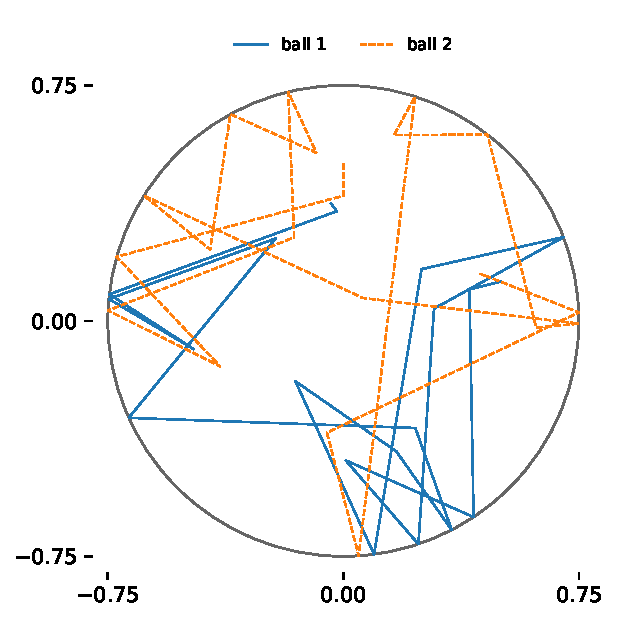
\includegraphics[width=0.5\textwidth]{figs/fishbowl}}
\caption{The paths of the two centres up to $t=10$, inside the circle
$|\bp| = 3/4$ to which they are confined.}
\end{figure}

Displacing a ball by $\delta$ moves the answer by about $\bowlamp\,\delta$,
so three to four digits are lost and fourteen working digits are enough.
At 25, 40 and 60 digits the computation returns $\bowllong$ each time, the
kinetic energy is still $1$ at the end, and I submit
\[
   \bowlanswer .
\]

\section{Conclusions}
The problems provided some fun, although Problems 2 and 5 are too closely
related: both are billiards, and the code for the first was recycled for the
second. That recycling is how the error in Section 6 got in. The rebound off
a curved wall carried over intact, and the one genuinely new ingredient ---
what happens when the two balls meet --- was the piece that never got a
derivation. An alternative problem is stated in the appendix.

\begin{table}[htb]
\centerline{\input{tables/answers}}
\caption{The five answers. Problem 5 is not the number submitted in 2005.}
\end{table}

The numbers come with a guarantee this time: each is reproduced by
\texttt{make check}, at two precisions or by two methods.

\begin{thebibliography}{9}
\bibitem{bornemann} F. Bornemann, D. Laurie, S. Wagon and J. Waldvogel,
\emph{The SIAM 100-Digit Challenge}, SIAM, Philadelphia, 2004.
\bibitem{trefethen} L. N. Trefethen and D. Bau, III, \emph{Numerical Linear
Algebra}, SIAM, Philadelphia, 1997.
\end{thebibliography}

\appendix
\section{A sixth problem}
There might be a tie at the end of the competition, and an additional
problem would then be published. Here is my suggestion.

\noindent\textbf{Problem.} \emph{Compute}
\begin{equation}\label{eq:integral}
   \int_0^1 \sin^2\bigl(\tan(\tan(\pi x))\bigr)\,dx .
\end{equation}
\vspace{-1.5\baselineskip}\diam

It was Brian Davies who pointed out that the evaluation would involve
serious difficulties both numerically and analytically. It is hard to
integrate this function on the real line, but a small step into the complex
plane gives us everything.

\subsection{Existence}
The function $f(x) = \sin^2(\tan(\tan(\pi x)))$ is undefined at some points
of $[0,1]$: the tangent has poles at $\pi/2 + k\pi$, so $f$ is undefined on
the countable set
\[
   X = \Bigl\{\tfrac{1}{\pi}\arctan\bigl(\tfrac{\pi}{2}+k\pi\bigr),
   \;k\in\mathbb{Z}\Bigr\}\cup\Bigl\{\tfrac{1}{2}\Bigr\} .
\]
Since $0 \le f \le 1$ on $[0,1]\setminus X$, the function is integrable and
the integral lies between $0$ and $1$. That is the last easy statement about
it on the real line: the graph oscillates without bound between consecutive
points of $X$, and a quadrature rule sees a sequence of essentially random
samples. Averaging over an equispaced grid of \integralgrid\ points returns
\integralnaive, which has one correct digit.

\subsection{The integrand in the complex plane}
From $e^{iz} = \cos z + i\sin z$,
\[
   \sin^2 z = \Bigl(\frac{e^{iz}-e^{-iz}}{2i}\Bigr)^2
   = \frac12 - \frac14\bigl(e^{2iz} + e^{-2iz}\bigr)
   = \frac12 - \frac12\cos(2z) ,
\]
and for real $x$ this gives the two real forms
\[
   \sin^2 x = \frac12 - \frac12\,\Re\,e^{2ix}
            = \frac12 - \frac12\,\Re\,e^{-2ix} ,
\]
which agree because $\Re \bar z = \Re z$. The functions $e^{2iz}$ and
$e^{-2iz}$ inside them continue to the whole plane; $\sin^2 z$ is not their
real part off the real line, and we shall not need it to be. The first is
bounded in the upper half-plane, where $|e^{2iz}| = e^{-2\Im z}\le 1$, and
the second in the lower half-plane. Write
\[
   f_c^{+}(x) = e^{+2i\tan(\tan(\pi x + ic))} , \qquad
   f_c^{-}(x) = e^{-2i\tan(\tan(\pi x - ic))} .
\]

\begin{lemma}\label{lem:tan}
The complex tangent maps the open upper half-plane into itself and the open
lower half-plane into itself.
\end{lemma}

\begin{proof}
Let $z = x+iy$. Then $\tan z = \sin z\,\overline{\cos z}/|\cos z|^2$, and
from
\[
   \sin z = \sin x\cosh y + i\cos x \sinh y , \qquad
   \cos z = \cos x\cosh y - i\sin x \sinh y
\]
the numerator has imaginary part
$\sinh y\cosh y(\sin^2 x + \cos^2 x) = \sinh y \cosh y$. Hence
\[
   \Im \tan z = \frac{\sinh y\,\cosh y}{|\cos z|^2} ,
\]
which has the sign of $y$. The poles of the tangent are real, so $\tan$ is
analytic on either open half-plane.
\end{proof}

By Lemma \ref{lem:tan} applied twice, $\tan(\tan z)$ is analytic and takes
values in the upper half-plane when $z$ does, so $f_0^{+}$ is analytic and
bounded by $1$ there. The same holds for $f_0^{-}$ below the axis.

\subsection{Dominated convergence}
For $c>0$ the function $f_c^{+}$ is continuous, and as $c \to 0$ it
converges to $e^{2i\tan(\tan(\pi x))}$ at every $x \in [0,1]\setminus X$,
hence almost everywhere. It is bounded by $1$ throughout, so dominated
convergence gives
\begin{equation}\label{eq:dct}
   \int_0^1 f_c^{+}\,dx \;\xrightarrow[c\to 0]{}\;
   \int_0^1 e^{2i\tan(\tan(\pi x))}\,dx ,
\end{equation}
and the same argument applies to $f_c^{-}$ below the axis.

\subsection{Cauchy's theorem}
The integrand $f_0^{+}$ is analytic in the open upper half-plane, so its
integral along a closed path there vanishes. Take the rectangle with corners
$ic_1$, $1+ic_1$, $1+ic_2$, $ic_2$ for $0 < c_1 < c_2$, with sides $A$, $C$
vertical and $B$, $D$ horizontal.

\begin{figure}[htb]
\centerline{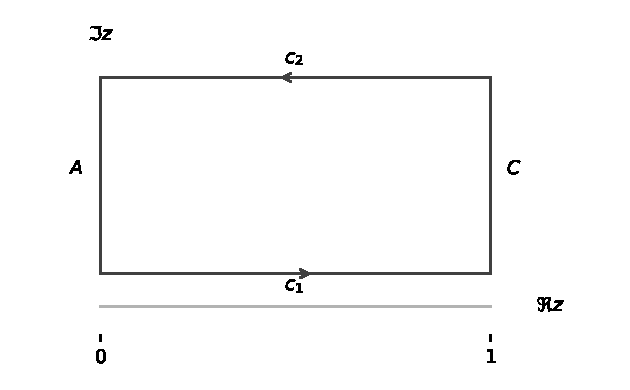
\includegraphics[width=0.5\textwidth]{figs/contour}}
\caption{The path of integration.}
\end{figure}

Since $\tan(\pi(x+1) + ic) = \tan(\pi x + ic)$, the integrand has period one
and the two vertical sides cancel. What is left is
\[
   \int_0^1 f_{c_1}^{+}\,dx = \int_0^1 f_{c_2}^{+}\,dx ,
\]
so the integral does not depend on the height of the contour:
\[
   \int_0^1 f_c^{+}\,dx = C \qquad \text{for all } c>0 ,
\]
and by \eqref{eq:dct} the same constant is the integral along the real axis.

The constant is now read off at the other end. As $c \to \infty$,
$\tan(\pi x + ic) \to i$ uniformly in $x$, so
$\tan(\tan(\pi x + ic)) \to \tan i = i\tanh 1$ uniformly and
\[
   f_c^{+}(x) \longrightarrow e^{2i\cdot i\tanh 1} = e^{-2\tanh 1} ,
\]
again uniformly. The integrands are bounded by $1$, so the integrals
converge to the same limit, and
\[
   C = e^{-2\tanh 1} .
\]
Keeping in mind how badly $f_0^{+}$ behaves on the real line, it is a
pleasant surprise that lifting the contour turns it into the simplest
function there is.

\begin{verbatim}
def closed_form(dps=40):
    """(1 - e^{-2 tanh 1})/2, the value the contour argument gives."""
    mp.mp.dps = dps
    return (1 - mp.e ** (-2 * mp.tanh(1))) / 2
\end{verbatim}


Putting the pieces together,
\[
   \int_0^1 \sin^2\bigl(\tan(\tan(\pi x))\bigr)\,dx
   = \frac12 - \frac12 e^{-2\tanh 1}
   = \integralvalue\ldots ,
\]
and the same argument applied to $f_c^{-}$ in the lower half-plane gives the
same number, as it must.

\subsection{A numerical confirmation}
The argument makes two claims that can be checked separately: that
$\int_0^1 f_c^{+}$ does not depend on $c$, and that its value is
$e^{-2\tanh 1}$. For $c>0$ the integrand is analytic and periodic, so the
trapezoid rule converges geometrically and a few dozen points suffice.

\begin{verbatim}
def lifted(c, n, dps=40):
    """The trapezoid rule for the integral of f_c^+ over one period.

    f_c^+(x) = exp(2i tan(tan(pi (x + i c)))) is analytic and has
    period 1 for c > 0, so the trapezoid rule converges
    geometrically and the answer must not depend on c at all.
    """
    mp.mp.dps = dps
    total = mp.mpc(0)
    for j in range(n):
        z = mp.mpf(j) / n + mp.mpc(0, 1) * c
        total += mp.e ** (2j * mp.tan(mp.tan(mp.pi * z)))
    return total / n
\end{verbatim}


At $c=1$ and $c=1/4$, sixty-four points already return
\integralshort\ldots, and at $c=1/20$, where the integrand is beginning to
oscillate, two hundred and fifty-six points do. The contour can be lowered
until the trapezoid rule fails, and the answer does not move until it does.

To ten digits, the sixth problem has the answer
\[
   \integralshort .
\]

\end{document}
